% =============================================================================
% Presentación de Defensa - Medidor de Latencias para Sistemas de
% Videovigilancia Críticos
% Guillermo Girón García - Universidad de Cádiz
% =============================================================================
\documentclass[aspectratio=169,11pt]{beamer}

% --- Theme ---
\usetheme{Madrid}
\usecolortheme{seahorse}
\setbeamertemplate{navigation symbols}{}
\setbeamertemplate{footline}[frame number]

% --- Packages ---
\usepackage[utf8]{inputenc}
\usepackage[T1]{fontenc}
\usepackage[spanish]{babel}
\usepackage{graphicx}
\usepackage{booktabs}
\usepackage{tikz}
\usetikzlibrary{shapes,arrows.meta,positioning,calc}
\usepackage{listings}
\usepackage{xcolor}

% --- Colors ---
\definecolor{ucablue}{RGB}{0,82,147}
\definecolor{ucagold}{RGB}{199,163,52}
\setbeamercolor{title}{fg=ucablue}
\setbeamercolor{frametitle}{fg=ucablue}
\setbeamercolor{structure}{fg=ucablue}

% --- Code style ---
\lstset{
    basicstyle=\ttfamily\scriptsize,
    breaklines=true,
    frame=single,
    backgroundcolor=\color{gray!10}
}

% --- Metadata ---
\title[Medidor de Latencias CCTV]{Medidor de Latencias para Sistemas de\\Videovigilancia Críticos}
\subtitle{Proyecto Fin de Carrera — Ingeniería Informática}
\author{Guillermo Girón García}
\institute{Escuela Superior de Ingeniería\\Universidad de Cádiz}
\date{2026}

% =============================================================================
\begin{document}

% --- PORTADA ---
\begin{frame}
\titlepage
\end{frame}

% --- ÍNDICE ---
\begin{frame}{Contenido}
\tableofcontents
\end{frame}

% =============================================================================
\section{Motivación}
% =============================================================================

\begin{frame}{¿Qué es la latencia en videovigilancia?}

\begin{columns}[T]
\begin{column}{0.55\textwidth}
\begin{itemize}
    \item Un sistema CCTV es \textbf{crítico} cuando el operador debe reaccionar en tiempo real ante lo que observa.
    \item La \textbf{latencia} es el retardo entre lo que ocurre frente a la cámara y lo que se muestra en el monitor.
    \item En entornos de seguridad (prisiones, infraestructuras críticas, fronteras), una latencia excesiva puede comprometer la respuesta ante incidentes.
\end{itemize}
\end{column}
\begin{column}{0.38\textwidth}
\begin{tikzpicture}[>=Stealth, node distance=1.2cm, font=\small]
    \node[draw, rounded corners, fill=blue!10, minimum width=2.2cm] (cam) {Cámara};
    \node[draw, rounded corners, fill=orange!10, minimum width=2.2cm, below=of cam] (red) {Red / Codec};
    \node[draw, rounded corners, fill=green!10, minimum width=2.2cm, below=of red] (mon) {Monitor};
    \draw[->, thick] (cam) -- (red);
    \draw[->, thick] (red) -- (mon);
    \node[right=0.3cm of red, text=red, font=\bfseries\scriptsize] {$\Delta t$};
\end{tikzpicture}
\end{column}
\end{columns}

\end{frame}

% =============================================================================
\begin{frame}{El problema}

\begin{alertblock}{No existe un instrumento portátil y económico}
para cuantificar de forma objetiva la latencia de un sistema de videovigilancia.
\end{alertblock}

\vspace{0.5cm}

\textbf{Soluciones existentes:}
\begin{itemize}
    \item Equipos de laboratorio (osciloscopios + generadores de patrones): costosos, no portátiles.
    \item Métodos manuales (cronómetro + vídeo): imprecisos, subjetivos.
    \item No hay estándar de medición para instalaciones ya desplegadas.
\end{itemize}

\vspace{0.3cm}
\textbf{Propuesta:} un dispositivo basado en Raspberry Pi que automatiza la medición mediante un LED estimulador y un fotosensor receptor.

\end{frame}

% =============================================================================
\section{Objetivos y alcance}
% =============================================================================

\begin{frame}{Objetivos del proyecto}

\begin{enumerate}
    \item Desarrollar el \textbf{software embebido} para un medidor de latencias portátil sobre Raspberry Pi 3.
    \item Proporcionar una \textbf{interfaz táctil} intuitiva y accesible (multilingüe, modos de visualización).
    \item Establecer una \textbf{cadena de compilación cruzada} completa para ARM64.
    \item Validar el software mediante \textbf{pruebas automatizadas} y emulación de la plataforma destino.
    \item Automatizar el despliegue con \textbf{scripts reproducibles} (un comando genera el binario de producción).
\end{enumerate}

\end{frame}

% =============================================================================
\begin{frame}{Evolución del alcance}

\begin{columns}[T]
\begin{column}{0.48\textwidth}
\textbf{Idea inicial:}
\begin{itemize}
    \item Producto de ingeniería completo
    \item Hardware + software + carcasa
    \item PCB dedicada, certificación
\end{itemize}
\end{column}
\begin{column}{0.48\textwidth}
\textbf{Alcance final:}
\begin{itemize}
    \item \textbf{Proyecto software completo}
    \item Arquitectura modular, tests automatizados
    \item Toolchain de compilación cruzada
    \item Documentación profesional
\end{itemize}
\end{column}
\end{columns}

\vspace{0.5cm}
\begin{block}{Decisión de ingeniería}
El componente software, por sí solo, constituye un proyecto de envergadura suficiente. Se priorizó entregar un producto software de calidad profesional.
\end{block}

\end{frame}

% =============================================================================
\section{Principio de medición}
% =============================================================================

\begin{frame}[fragile]{¿Cómo se mide la latencia?}

\begin{center}
\begin{tikzpicture}[>=Stealth, node distance=2cm, font=\small, thick]
    % Nodes
    \node[draw, rounded corners, fill=yellow!20, minimum width=2cm, minimum height=1cm] (led) {LED};
    \node[draw, rounded corners, fill=blue!15, minimum width=2cm, minimum height=1cm, right=2cm of led] (cam) {Cámara};
    \node[draw, rounded corners, fill=gray!15, minimum width=2cm, minimum height=1cm, right=2cm of cam] (mon) {Monitor};
    \node[draw, rounded corners, fill=green!20, minimum width=2cm, minimum height=1cm, align=center, right=2cm of mon] (sensor) {Fotosensor\\+ ADC};
    
    % RPi below
    \node[draw, rounded corners, fill=red!10, minimum width=3cm, minimum height=0.8cm, below=1.5cm of $(led)!0.5!(sensor)$] (rpi) {Raspberry Pi};
    
    % Arrows
    \draw[->, dashed, orange] (led) -- node[above]{\scriptsize luz} (cam);
    \draw[->] (cam) -- node[above]{\scriptsize señal} (mon);
    \draw[->, dashed, green!60!black] (mon) -- node[above]{\scriptsize luz} (sensor);
    \draw[<->, red] (rpi) -- (led);
    \draw[<->, red] (rpi) -- (sensor);
    
    % Time annotation
    \draw[<->, thick, blue] ([yshift=-0.5cm]led.south) -- node[below, font=\bfseries\small, text=blue]{$\Delta t$ = Latencia medida} ([yshift=-0.5cm]sensor.south);
\end{tikzpicture}
\end{center}

\vspace{0.3cm}
\begin{enumerate}
    \item La RPi enciende el LED → se registra $t_1$
    \item La cámara capta la luz y la transmite al monitor
    \item El fotosensor detecta la luz en el monitor → el ADC (ADS1115) digitaliza la señal → se registra $t_2$
    \item $\text{Latencia} = t_2 - t_1$
\end{enumerate}

\end{frame}

% =============================================================================
\section{Arquitectura del software}
% =============================================================================

\begin{frame}{Arquitectura: Core / GUI}

\begin{columns}[T]
\begin{column}{0.45\textwidth}
\textbf{Core} (sin dependencias GUI):
\begin{itemize}
    \item \texttt{AppSettings} — configuración (singleton)
    \item \texttt{SensorOperator} — LED + fotosensor
    \item \texttt{JsonOperator} — persistencia JSON
    \item \texttt{dataModel} — estructuras de datos
\end{itemize}

\vspace{0.3cm}
\textbf{GUI} (Qt Widgets):
\begin{itemize}
    \item 7 pantallas independientes
    \item \texttt{QStackedWidget} como navegador
    \item Signals/Slots entre pantallas
\end{itemize}
\end{column}
\begin{column}{0.5\textwidth}
\begin{tikzpicture}[font=\scriptsize, node distance=0.25cm, >=Stealth]
    \node[draw, fill=ucablue!15, rounded corners, minimum width=4cm] (mw) {MainWindow (QStackedWidget)};
    \node[draw, fill=green!10, rounded corners, below=0.2cm of mw, minimum width=4cm] (home) {HomeScreen};
    \node[draw, fill=green!10, rounded corners, below=0.12cm of home, minimum width=4cm] (meas) {MeasureScreen};
    \node[draw, fill=green!10, rounded corners, below=0.12cm of meas, minimum width=4cm] (sett) {SettingsScreen};
    \node[draw, fill=green!10, rounded corners, below=0.12cm of sett, minimum width=4cm] (reg) {RegistryScreen};
    \node[draw, fill=green!10, rounded corners, below=0.12cm of reg, minimum width=4cm] (regd) {RegistryDisplayScreen};
    \node[draw, fill=green!10, rounded corners, below=0.12cm of regd, minimum width=4cm] (help) {HelpScreen};
    \node[draw, fill=green!10, rounded corners, below=0.12cm of help, minimum width=4cm] (helpi) {HelpInfoScreen};
    
    \node[draw, fill=orange!10, rounded corners, right=0.6cm of sett, minimum width=2cm] (core) {Core};
    \draw[->] (meas.east) -- (core.west);
    \draw[->] (sett.east) -- (core.west);
    \draw[->] (reg.east) -- (core.west);
\end{tikzpicture}
\end{column}
\end{columns}

\end{frame}

% =============================================================================
\section{Interfaz de usuario}
% =============================================================================

\begin{frame}{Pantalla de inicio}
\begin{center}
    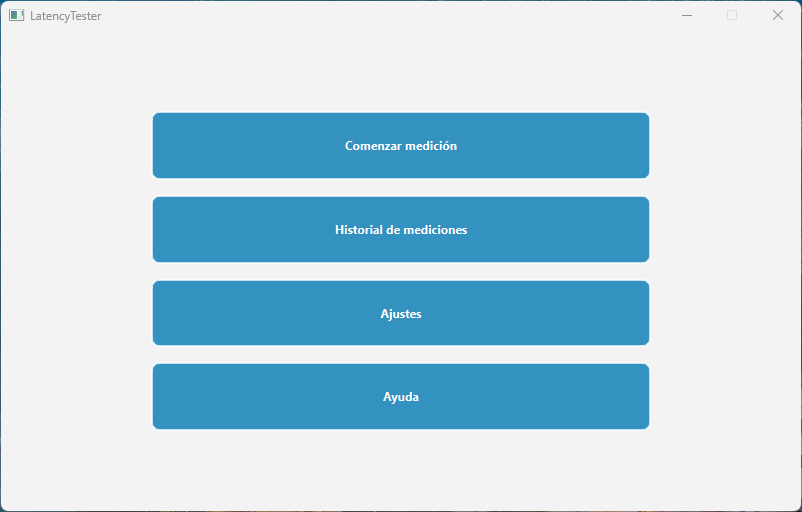
\includegraphics[height=0.75\textheight]{home_screen.png}
\end{center}
\end{frame}

\begin{frame}{Pantalla de medición}
\begin{center}
    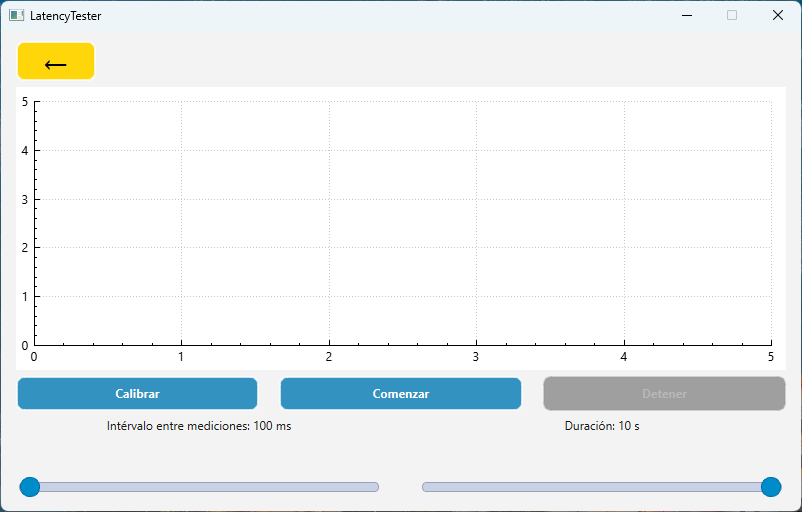
\includegraphics[height=0.75\textheight]{take_measure_screen.png}
\end{center}
\end{frame}

\begin{frame}{Visualización de resultados}
\begin{center}
    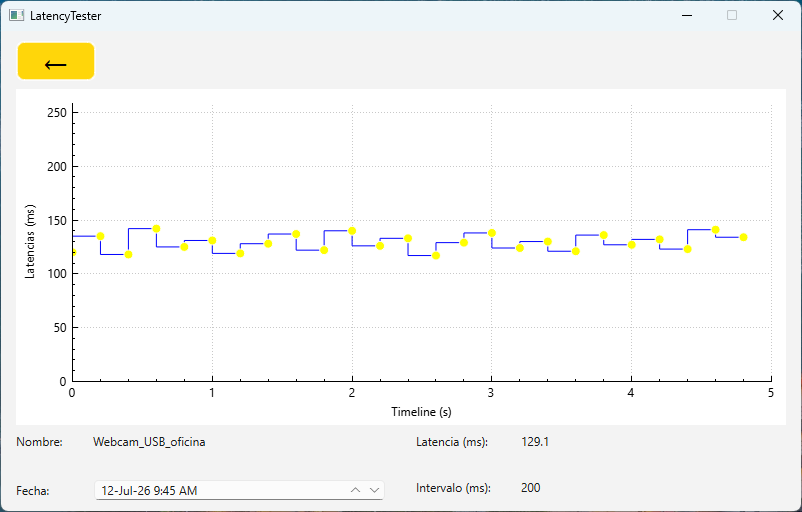
\includegraphics[height=0.75\textheight]{displayer_screen.png}
\end{center}
\end{frame}

% =============================================================================
\section{Toolchain de compilación cruzada}
% =============================================================================

\begin{frame}{El mayor reto técnico: la Toolchain ARM64}

\begin{center}
\begin{tikzpicture}[font=\scriptsize, >=Stealth, node distance=0.5cm]
    \node[draw, fill=blue!10, rounded corners, minimum width=2.3cm, minimum height=0.6cm] (gcc) {GCC 13 ARM64};
    \node[draw, fill=purple!10, rounded corners, minimum width=2.3cm, minimum height=0.6cm, right=0.4cm of gcc] (qt) {Qt 6.11.1 ARM64};
    \node[draw, fill=yellow!10, rounded corners, minimum width=2.3cm, minimum height=0.6cm, right=0.4cm of qt] (sys) {Sysroot (Docker)};
    
    \node[draw, fill=red!10, rounded corners, minimum width=8.5cm, minimum height=0.6cm, below=0.4cm of qt] (build) {\texttt{build-arm64.sh --production}};
    
    \node[draw, fill=green!15, rounded corners, minimum width=4cm, minimum height=0.6cm, below=0.4cm of build] (bin) {\textbf{LatencyTester} (ARM64 ELF)};
    
    \draw[->] (gcc.south) -- (build.north);
    \draw[->] (qt.south) -- (build.north);
    \draw[->] (sys.south) -- (build.north);
    \draw[->, thick] (build.south) -- (bin.north);
\end{tikzpicture}
\end{center}

\vspace{0.1cm}
\textbf{Problemas resueltos:}
\begin{columns}[T]
\begin{column}{0.48\textwidth}
\begin{itemize}
    \item qmake incompatible con QEMU
    \item GLIBC mismatch → linker \texttt{lld}
    \item GCC 12 sin \texttt{<format>} → GCC 13
\end{itemize}
\end{column}
\begin{column}{0.48\textwidth}
\begin{itemize}
    \item Qt sin prebuilt ARM64 → compilar desde fuente
    \item libgpiod v2 sin paquete → compilar desde fuente
    \item pigpio ausente en repos → compilar desde fuente
\end{itemize}
\end{column}
\end{columns}

\end{frame}

% =============================================================================
\begin{frame}[fragile]{Automatización total}

\begin{block}{Un solo comando genera el binario de producción}
\begin{lstlisting}
cd LatencyTester/Scripts/Linux
./setup-toolchain.sh
\end{lstlisting}
\end{block}

\vspace{0.2cm}

\textbf{8 pasos automatizados:}
\begin{columns}[T]
\begin{column}{0.48\textwidth}
\begin{enumerate}
    \item Dependencias host (GCC 13, lld)
    \item Emulación ARM64 (QEMU)
    \item Imagen Docker ARM64
    \item Extracción de sysroot
\end{enumerate}
\end{column}
\begin{column}{0.48\textwidth}
\begin{enumerate}
    \setcounter{enumi}{4}
    \item Qt 6.11.1 desde fuente
    \item libgpiod v2.2 + C++ bindings
    \item pigpio desde fuente
    \item Binario de producción
\end{enumerate}
\end{column}
\end{columns}

\vspace{0.2cm}
\textbf{Alternativa portable} (Linux/Windows/macOS): \texttt{docker-production.sh build}

\end{frame}

% =============================================================================
\section{Pruebas y validación}
% =============================================================================

\begin{frame}{Estrategia de validación en tres niveles}

\begin{table}
\centering
\begin{tabular}{lll}
\toprule
\textbf{Nivel} & \textbf{Herramienta} & \textbf{Resultado} \\
\midrule
Pruebas unitarias & QTest (147 tests) & 145 pass, 2 skip \\
Análisis de memoria & ASan + Valgrind & 0 fugas reales \\
Plataforma destino & Docker ARM64 + VNC & Correcto \\
\bottomrule
\end{tabular}
\end{table}

\vspace{0.5cm}

\begin{columns}[T]
\begin{column}{0.48\textwidth}
\textbf{10 suites de test:}
\begin{itemize}
    \item 4 suites Core (datamodel, settings, JSON, sensor)
    \item 6 suites GUI (todas las pantallas)
\end{itemize}
\end{column}
\begin{column}{0.48\textwidth}
\textbf{Bugs detectados por tests:}
\begin{itemize}
    \item Lógica \texttt{if} invertida (JsonOperator)
    \item Memory leak 448B/llamada (ASan)
    \item Colons en filenames (Windows)
\end{itemize}
\end{column}
\end{columns}

\end{frame}

% =============================================================================
\section{Conclusiones}
% =============================================================================

\begin{frame}{Conclusiones}

\begin{itemize}
    \item Se ha desarrollado un \textbf{software embebido completo} para un medidor de latencias de videovigilancia, validado en dos arquitecturas (x86-64 y ARM64).
    
    \item La configuración de la \textbf{toolchain de compilación cruzada} fue el mayor reto técnico — 6+ problemas encadenados resueltos iterativamente.
    
    \item El resultado es un flujo de trabajo \textbf{completamente automatizado y reproducible}: un solo script produce un binario de producción desde un sistema limpio.
    
    \item El dispositivo propuesto llena un \textbf{vacío real} en el mercado de la videovigilancia crítica: no existía un instrumento portátil, económico y autónomo para esta medición.
\end{itemize}

\vspace{0.3cm}
\begin{block}{Estado actual}
Software completamente funcional y validado. Pendiente: integración con hardware real en Raspberry Pi física.
\end{block}

\end{frame}

% =============================================================================
\section{Trabajo futuro}
% =============================================================================

\begin{frame}{Trabajo futuro}

\begin{columns}[T]
\begin{column}{0.32\textwidth}
\textbf{Hardware}
\begin{itemize}
    \item Validación en RPi real
    \item PCB dedicada
    \item Carcasa industrial
    \item Certificación CE
\end{itemize}
\end{column}
\begin{column}{0.32\textwidth}
\textbf{Software}
\begin{itemize}
    \item Exportación CSV/PDF
    \item Monitorización continua
    \item Actualización OTA
    \item Conectividad WiFi
\end{itemize}
\end{column}
\begin{column}{0.32\textwidth}
\textbf{Evolución}
\begin{itemize}
    \item Migración a RPi 4/CM4
    \item Gestión remota multi-dispositivo
    \item Dashboard web
\end{itemize}
\end{column}
\end{columns}

\end{frame}

% =============================================================================
\begin{frame}{}
\begin{center}
\vspace{1cm}
{\Huge\textcolor{ucablue}{Gracias}}

\vspace{1cm}
{\large Pasamos a la demostración}

\vspace{1cm}
{\small Guillermo Girón García — Universidad de Cádiz, 2026}
\end{center}
\end{frame}

\end{document}
